\chapter{Risultati e Valutazioni}
\label{cap:nomePrimoCapitoloTesi}
\lhead{\textbf{\rightmark}}

\indent{
	In questo capitolo sono presenti diverse analisi dei nevi, utilizzando l'applicazione "Naevus" e verificando se i dati sono computati correttamente e se le procedure di segmentazione e messa in evidenza dei bordi sono eseguite con successo.
	In seguito sono presentati test in diverse situazioni di luce, messa a fuoco e con presenza o meno di peli spessi o sottili.
	Saranno effettuati tre test per ogni situazione.
\newpage
\section{Analisi dei nevi }
\subsection{Analisi con luce naturale senza peli }
L'analisi del nevo con poca luce ha mostrato come sia di fondamentale importanza lanciare l'analisi in condizioni di luce ottimali se si vuole ottenere un risultato consistente e utilizzabile per il dermatologo. Il tempo impiegato per l'intera analisi sulla macchina server \footnote{vedi Appendice B} è di 5.2 secondi per frame.
\begin{figure}[h]
	\begin{center}
		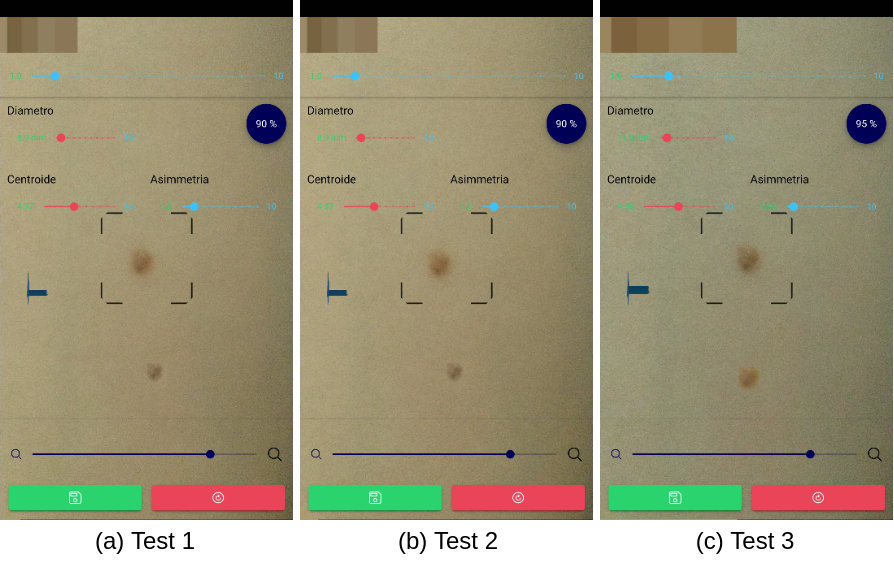
\includegraphics[scale=0.45]{figure/capitolo7/test1.png}
	\end{center}
	\caption{Analisi del nevo con poca luce}	
\end{figure}
\newpage
\subsection{Analisi con flash e luce artificiale senza peli} 
L'analisi del nevo con un livello ottimale di luce e con il flash del device acceso ha mostrato come si ottengano risultati soddisfacenti e consistenti anche in ulteriori analisi.
\newline
I risultati in Figura 7.2 sono molto simili tra di loro e discostano di pochi punti per ogni feature.
Questa analisi ha dimostrato la necessità di una buona illuminazione quando si analizza il nevo.
La media dei tempi per l'analisi è di 5 secondi. 
\begin{figure}[h]
	\begin{center}
		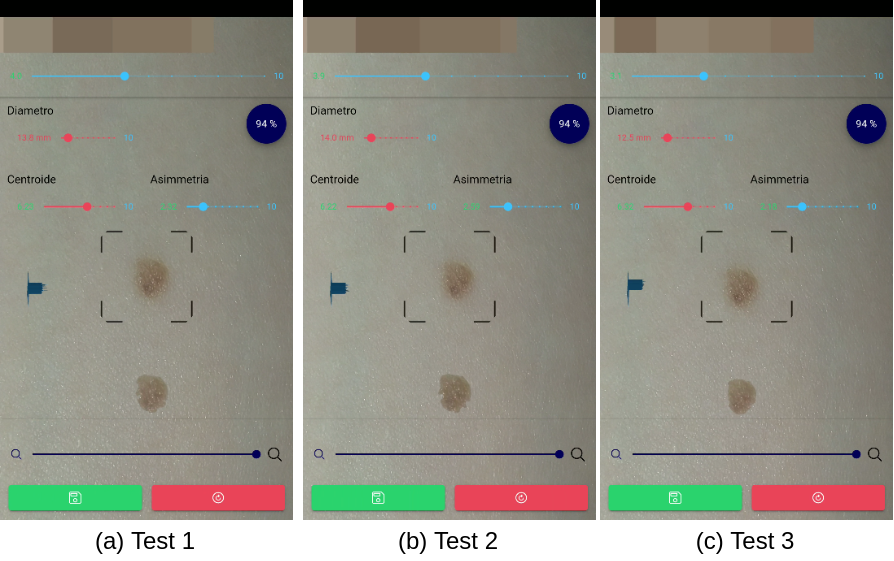
\includegraphics[scale=0.45]{figure/capitolo7/test2.png}
	\end{center}
	\caption{Analisi del nevo con flash e luce artificiale}	
\end{figure}
\newpage
\subsection{Analisi con flash e luce artificiale con peli} 
Come visto in precedenza, nel caso in cui il nevo sia coperto da peli, sarà necessario applicare l'algoritmo di \textbf{rimozione peli}.
Nella Figura 7.3 si nota che nel primo test di analisi (a) la segmentazione non è riuscita a selezionare il nevo correttamente, mentre aumentando al massimo lo zoom sul nevo nei test (b) e (c) i risultati ottenuti sono stati soddisfacenti e simili tra loro.
Il tempo impiegato per l'intera analisi sulla macchina server \footnote{vedi Appendice B} è di 6.5 secondi per frame.
\begin{figure}[h]
	\begin{center}
		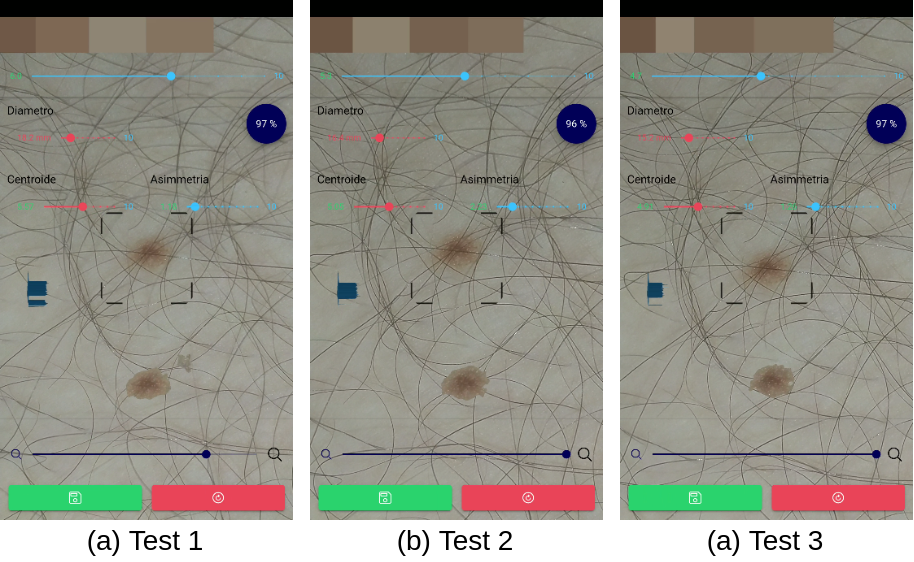
\includegraphics[scale=0.45]{figure/capitolo7/test3.png}
	\end{center}
	\caption{Analisi del nevo con peli}	
\end{figure}
\newpage
\subsection{Analisi nevo < 1cm con flash e luce artificiale} 
L'analisi di nevi di dimensione inferiore a 1 centimetro è efficace in condizioni di luce ottimale.
In Figura 7.4 l'analisi di un nevo di dimensione < di 8 millimetri.
Il tempo impiegato per l'intera analisi sulla macchina server \footnote{vedi Appendice B} è di 4.1 secondi per frame.
\begin{figure}[h]
	\begin{center}
		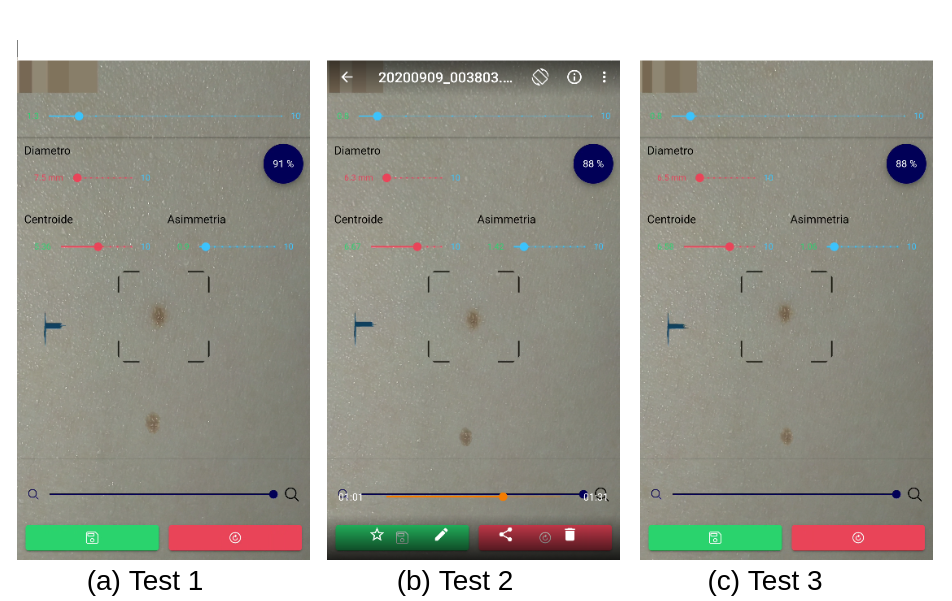
\includegraphics[scale=0.45]{figure/capitolo7/test4.png}
	\end{center}
	\caption{Analisi di un nevo nevo < 1cm}	
\end{figure}
\newpage
\subsection{Esempi di analisi errata}
Le analisi che si sono rivelate errate ed inconsistenti sono dovute ad alcuni errori di scatto da parte dell'utente ed impossibilità dell'algoritmo di segmentare correttamente il nevo.
\newline
Nella Figura 7.5 (a) la luce non era ottimale nelle direzioni opposte al nevo traendo in inganno l'algoritmo di segmentazione che non è riuscito ad individuare correttamente il nevo.
\newline
Nella Figura 7.5 (b) la posizione dello smartphone è inclinata rispetto al nevo e questo non ha permesso al classificatore di individuare il nevo correttamente.
\newline
Nella Figura 7.5 (c) la sfocatura data dallo zoom non ha permesso all'algoritmo di distinguere la pelle dal nevo.
\begin{figure}[h]
	\begin{center}
		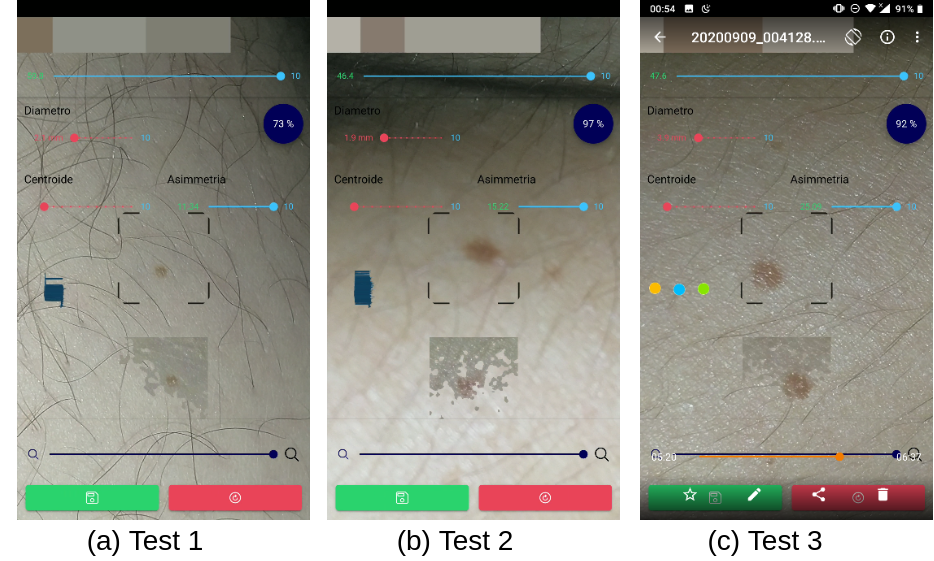
\includegraphics[scale=0.4]{figure/capitolo7/test5.png}
	\end{center}
	\caption{Esempi analisi errata }	
\end{figure}
\newpage
\subsection{Effettuare un'analisi ottimale}
Per ottenere risultati soddisfacenti ed utilizzabili in ambito clinico bisogna assicurare che i seguenti requisiti pre-analisi siano soddisfatti:
\begin{itemize}
	\item Lo smartphone deve essere posto perpendicolarmente al nevo. (Figura 7.6)
	\item La luce deve essere ottimale in ogni direzione opposta al nevo.
	\item Il nevo deve avere un colore, o un range di colori, più scuri rispetto al colore della pelle.
\end{itemize}

\begin{figure}[h]
	\begin{center}
		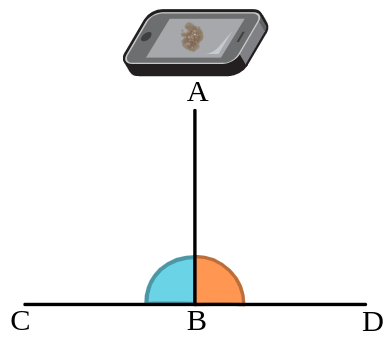
\includegraphics[scale=0.45]{figure/capitolo7/perpendicolare.png}
	\end{center}
	\caption{Smartphone posto perpendicolarmente rispetto al nevo.}	
\end{figure}
Quando una di queste tre condizioni non viene soddisfatta, i risultati possono essere non corretti e ricevere un messaggio di errore da parte dell'applicazione.
}